\documentclass[tikz,border=12pt]{standalone}
\usepackage[T1]{fontenc}
\usepackage{mathpazo}
\usepackage{amsmath,amssymb}
\usetikzlibrary{arrows.meta, positioning, calc, fit, decorations.pathreplacing}

\definecolor{stblue}{HTML}{7B97AD}
\definecolor{rwgold}{HTML}{B8995E}
\definecolor{sage}{HTML}{7A9A7E}
\definecolor{dkbrown}{HTML}{3D3530}
\definecolor{wmgray}{HTML}{7B7067}
\definecolor{cream}{HTML}{F9F6F0}
\definecolor{border}{HTML}{D4C9B8}
\definecolor{terracotta}{HTML}{C47A6A}
\definecolor{lavender}{HTML}{907EA0}

\begin{document}
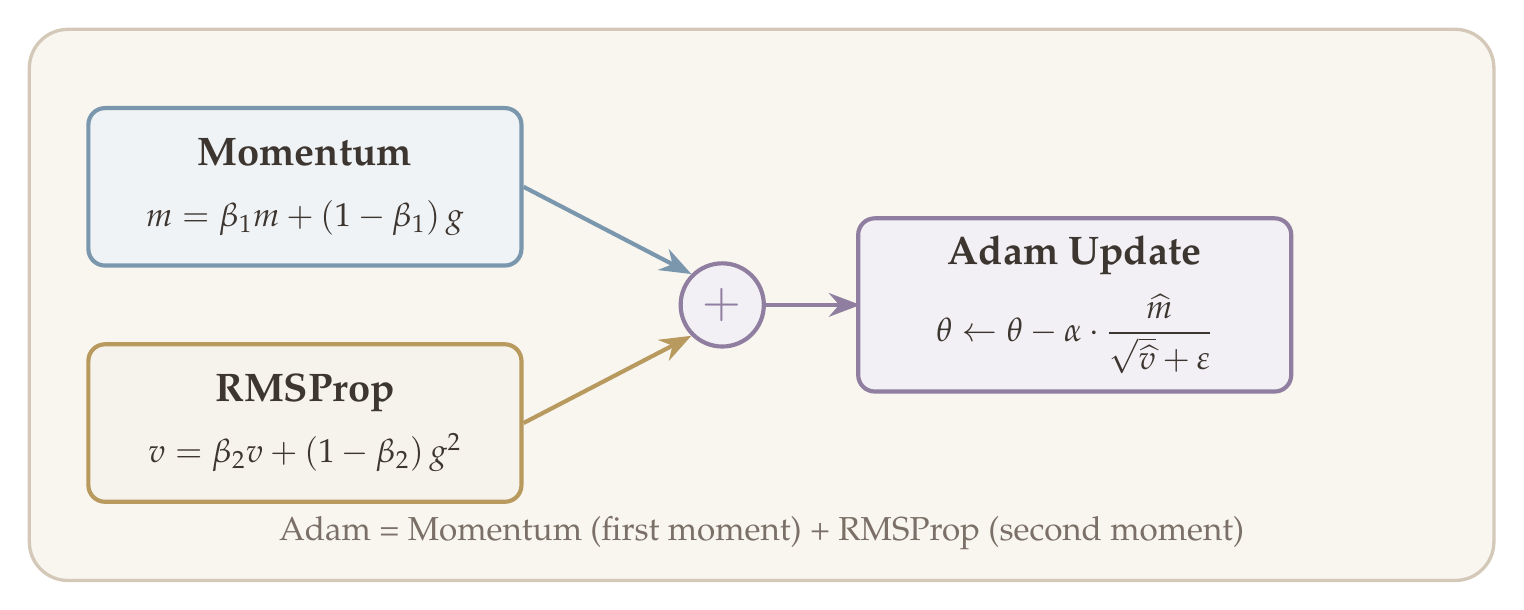
\begin{tikzpicture}[>={Stealth[length=4mm, width=3mm]}, line width=1.5pt]

% Background
\fill[cream, rounded corners=14pt] (-0.3,-1.0) rectangle (18.3,6.0);
\draw[border, line width=1.2pt, rounded corners=14pt] (-0.3,-1.0) rectangle (18.3,6.0);

% Momentum box
\node[draw=stblue, line width=1.5pt, fill=stblue!12, rounded corners=6pt,
      minimum width=5.5cm, minimum height=2.0cm, text=dkbrown, font=\Large,
      align=center] (momentum) at (3.2,4.0) {\textbf{Momentum}\\[4pt]
      {\large $m = \beta_1 m + (1-\beta_1)\,g$}};

% RMSProp box
\node[draw=rwgold, line width=1.5pt, fill=rwgold!12, rounded corners=6pt,
      minimum width=5.5cm, minimum height=2.0cm, text=dkbrown, font=\Large,
      align=center] (rmsprop) at (3.2,1.0) {\textbf{RMSProp}\\[4pt]
      {\large $v = \beta_2 v + (1-\beta_2)\,g^2$}};

% Merge circle
\node[draw=lavender, line width=1.5pt, fill=lavender!12, circle,
      inner sep=4pt, font=\LARGE\bfseries, text=lavender] (merge) at (8.5,2.5) {$+$};

% Arrows from boxes to merge
\draw[stblue, ->, line width=1.5pt] (momentum.east) -- (merge.north west);
\draw[rwgold, ->, line width=1.5pt] (rmsprop.east) -- (merge.south west);

% Arrow to Adam box
\draw[lavender, ->, line width=1.5pt] (merge.east) -- ++(1.2,0);

% Adam update box
\node[draw=lavender, line width=1.5pt, fill=lavender!12, rounded corners=6pt,
      minimum width=5.5cm, minimum height=2.2cm, text=dkbrown, font=\Large,
      align=center, anchor=west] (adam) at (10.2,2.5) {\textbf{Adam Update}\\[6pt]
      {\large $\theta \leftarrow \theta - \alpha \cdot \dfrac{\widehat{m}}{\sqrt{\widehat{v}} + \varepsilon}$}};

% Caption
\node[text=wmgray, font=\large] at (9.0,-0.4) {Adam = Momentum (first moment) + RMSProp (second moment)};

\end{tikzpicture}
\end{document}
